\documentclass[12pt,a4paper,UTF8]{article}
\usepackage{ctex} % Chinese support
\usepackage{graphicx} % Insert images
\usepackage{subfigure}
\usepackage{float}
\usepackage{listings} % Print source code
\usepackage{color} % Color support
\usepackage{booktabs} % Professional table support
\usepackage{pdflscape} % Landscape pages support in PDF
\usepackage{hyperref} % Hypertext links support for cross-referencing
\usepackage{amsmath,mathtools}
\usepackage{amssymb}
\usepackage{ulem} % strikethrough
\usepackage{diagbox} % diagonal in tabular
\usepackage{multirow} % multirow in tabular
% \usepackage{changepage} % whole paragraph indent

% Customize hyperref format (it's set to no special format here)
\hypersetup{hidelinks}

% Declare directories to search for graphics files for graphicx
\graphicspath{{figures/}}

% Define source code style for listings
\lstdefinestyle{verilog-style}{
	language=Verilog,
	basicstyle=\ttfamily\footnotesize,
	keywordstyle=\bfseries\color[rgb]{0, 0, 1},
	identifierstyle=\color[rgb]{0.5, 0.3, 0.1},
	stringstyle=\color[rgb]{0.6, 0.1, 0.1},
	commentstyle=\itshape\color[rgb]{0.05, 0.5, 0.05},
	backgroundcolor=\color[gray]{0.95},
	numbers=left,
	numbersep=5pt,
	numberstyle=\color[gray]{0.6},
	breaklines=true
}

\newcommand{\reporttitle}[2]{
  \LARGE\textsf{#1}\quad\underline{\makebox[12em]{#2}}
}

\newcommand{\reportinfo}[2]{
  \large\makebox[4em]{\textsf{#1}}\quad\underline{\makebox[18em]{#2}}
}

\begin{document}
\begin{titlepage}
  \centering
  \vspace*{\fill}
  {\Huge\textsf{数字电路与数字系统实验}} \\ [100pt]
  \reportinfo{实验名称}{exp03 加法器} \\ [10pt]
  \reportinfo{院系}{计算机科学与技术系} \\ [10pt]
  \reportinfo{学生姓名}{} \\ [10pt]
  \reportinfo{学号}{} \\ [10pt]
  \reportinfo{班级}{数字电路与数字系统实验1班} \\ [10pt]
  \reportinfo{邮箱}{} \\ [10pt]
  \reportinfo{实验时间}{2020 年 9 月 18 日} \\ [10pt]
  \vspace*{\fill}
\end{titlepage}
\tableofcontents
\newpage

\section{实验目的}
\begin{itemize}
  \item 复习加法器的原理和学习ALU的设计方式
  \item 实现加减运算的进位标志、溢出标志、零标志
  \item 实现简单ALU的逻辑运算功能
  \item 学习Verilog中task功能的使用
  \item 训练思维的细致性和全面性,测试程序时
        要进行尽可能全面的计算和验证
\end{itemize}

\section{实验原理}
\begin{itemize}
  \item 有符号数补码的加法器和标志信号的原理:\\
        $result = in\_x + in\_y$
  \item 有符号数减法是对减数求补,再与被减数相加
        得到结果:\\ $result = in\_x + \sim in\_y + 1$

  \item 进位位的原理和表达式: \\
        对于有符号数补码加法,进位位这样设置:\\
        $\{carry, result\} = in\_x + in\_y$ \\
        其中x, y, result是n位补码,carry是进位位。 \\
        对于有符号数补码减法,进位位有两种相反的设置方法:\\
        \begin{subequations}
          \begin{equation}
            \{carry, temp\} = \sim(in\_x + \sim in\_y + 1)
            \label{cf1}
          \end{equation}
          \begin{equation}
            \{carry, temp\} = in\_x + \sim in\_y + 1
            \label{cf2}
          \end{equation}
        \end{subequations}
        也就是说,减法的进位位是对于其转化成的加法来设置的。
        第一种(公式\eqref{cf1})将加法的进位输出取反,
        以此作为进位位。第二种(公式\eqref{cf2})直接
        将加法的进位输出作为进位位。 \\
        从无符号数的层面上来理解,这里的进位位和
        无符号数运算的进/借位标志是一致的。我们先要
        把补码运算的两个操作数向量转换成两个无符号数。
        对于加法,若两个无符号数相加进位,则进位位置1。
        对于减法,若两个无符号数相减产生借位,即被减数
        小于减数,则按第一种方法会将进位位置1;否则置0。
        若按第二种方法,则在做减法时进位位正好与
        第一种方法相反。 \\
        \begin{figure}[H]
          \centering
          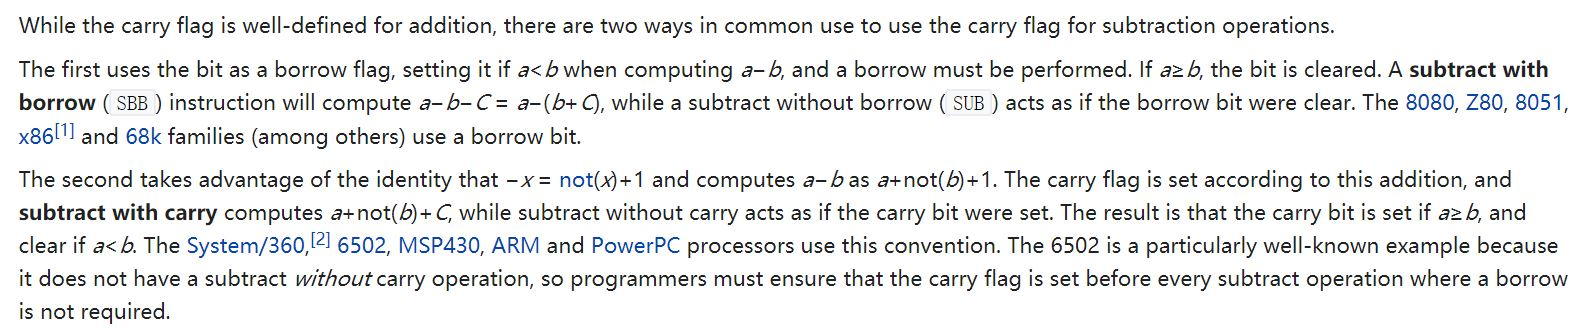
\includegraphics[width=1\textwidth]{cf_def.JPG}
          \caption{维基百科对进位位CF的解释}
          \label{cf_def}
        \end{figure}
        由于实验题目中未说明需要实现的加减法器采用哪种
        进位位的实现方法,而且我在一开始研究实验时并不知道
        进位位还有第二种的定义。因此我就按照公式\eqref{cf1}
        编写实验代码和测试文件。直到做到思考题2时,我才觉得
        进位位有问题,于是去询问老师,然后得知本实验采用
        第二种方法,即按照公式\eqref{cf2}设置进位位:
        \begin{figure}[H]
          \centering
          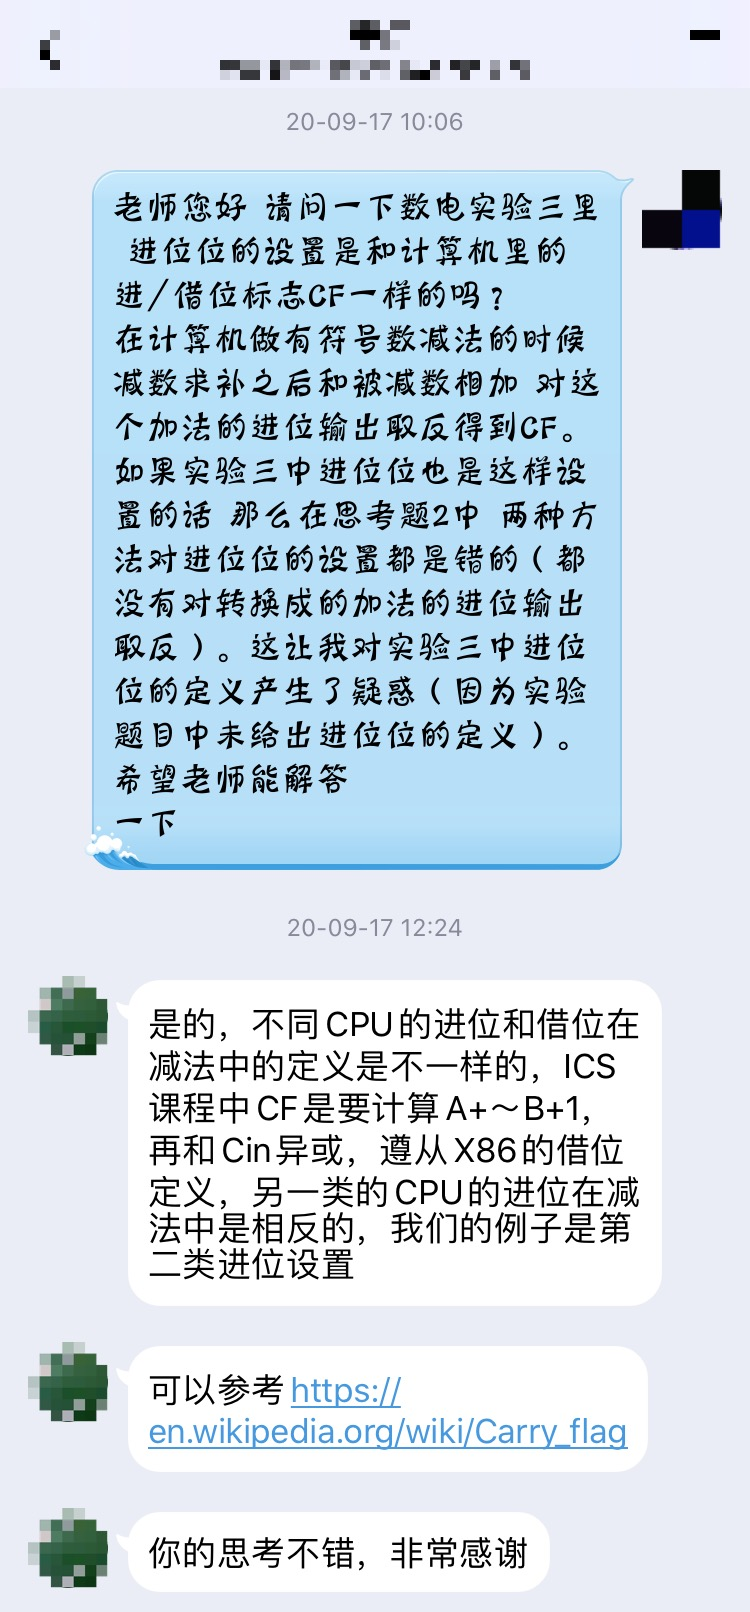
\includegraphics[width=0.6\textwidth]{cf_explanation.JPG}
          \caption{本实验采用的进位位设置}
          \label{cf_explanation}
        \end{figure}

  \item 溢出位的原理和表达式;\\
        对于加法,表达式在实验题目中已给出:\\
        \begin{equation}
          \begin{aligned}
            overflow = & (in\_x[n-1] == in\_y[n-1])       \\
                       & \&\& (result[n-1] != in\_x[n-1])
          \end{aligned}
        \end{equation}
        画张表格来理解这个式子:\\
        \\
        \begin{tabular}[H]{c|c|c|c|c}
          加法                  & A    & B & result & 是否溢出 \\ \hline
          \multirow{2}*{符号位} & 0    & 0 & 1
                                & 溢出                         \\ \cline{2-5}
                                & 1    & 1 & 0      & 溢出     \\
        \end{tabular} \\
        \\
        从整数运算层面来理解:若两个正数相加得负数,
        或者两个负数相加得正数,则溢出。\\
        对于减法,则和前文计算运算结果和计算进位位
        一样,把减法转换成加法,再套用实验题目中
        给出的溢出位公式。其中要注意的是,在溢出位
        计算公式中,in\_y对应的是减法中的
        减数取反,而不是减数取反加一。这两种取值的
        唯一区别在于减数是$-2^{n-1}$的情况,
        这个数的相反数是正数,符号位应是0,而它取反加一
        的结果仍是它本身,符号位是1。
  \item 零标志位的情况很简单,只要根据计算结果判断即可
  \item 有符号数补码的逻辑运算的原理
\end{itemize}

\section{实验环境/器材}
\begin{itemize}
  \item Quartus编辑器和DE10-Standard开发平台
  \item FPGA开发板
\end{itemize}

\section{程序代码+实验步骤/过程+测试方法}

\subsection{实验3.3.1 简单加减法运算器的设计}
\subsubsection{4位补码的加减运算}
计算加减法结果的代码是不难写的,难点在于进位位和
溢出位。需要根据实验题目所给出的公式,考虑很多情况,
不断试错。写了之后发现还是思考题2方法一的代码
更加优雅,于是照搬如下:
\begin{lstlisting}[style=verilog-style]
module ALU_adder(A, B, Cin, Y);
	input [3:0] A, B;
	input Cin;
	output [6:0] Y;
	wire [3:0] t_no_Cin;

	assign t_no_Cin = {4{Cin}} ^ B;
	assign Y[4:0] = A + t_no_Cin + Cin; // { carry, result}
	assign Y[5] = (A[3] == t_no_Cin[3]) 
	            && (A[3] != Y[3]); // overflow
	assign Y[6] = ~(| Y[3:0]); // zero 
endmodule  
\end{lstlisting}

\subsubsection{测试代码中如何计算正确的值}
首先我们需要知道补码加法的原理:\\
\indent $\forall -2^{n-1}\leqslant x, y\leqslant 2^{n-1}-1, $
\begin{equation}
  x+y=\begin{cases}
    x+y-2^n, & 2^{n-1}\leqslant x+y            \\
    x+y,     & -2^{n-1}\leqslant x+y < 2^{n-1} \\
    x+y+2^n, & x+y < -2^{n-1}
  \end{cases}
\end{equation}

接下来确定一下要添加哪些变量:
\begin{itemize}
  \item 对于A,B,Cin,需要嵌套三层循环,
        分别对应循环变量i, j, k
  \item u\_a和u\_b是向量A和B对应的无符号数
  \item sum\_ab是i+j或i-j的结果,根据Cin来确定
        是i+j还是i-j
  \item out\_y是4位向量,表示加减法器应该输出的值
  \item 需要计算out\_y, cf, of, zf的正确的值,
        从而传入到task中进行测试
\end{itemize}

先测试做加法的情况:

当$x+y \geqslant 2^{n-1}$时,三个标志位都是确定的:
\begin{lstlisting}[style=verilog-style]
if (sum_ab >= 8) begin
      out_y = sum_ab - 16;
      cf = 0;
      of = 1;
      zf = 0;
end
\end{lstlisting}

当$x+y < -2^{n-1}$时,只有零标志位需要判断一下:
\begin{lstlisting}[style=verilog-style]
else if (sum_ab < -8) begin
      out_y = sum_ab + 16;
      cf = 1;
      of = 1;
      zf = (out_y == 0) ? 1 : 0;
end      
\end{lstlisting}

当$-2^{n-1}\leqslant x+y < 2^{n-1}$时,除了
需要对零标志位进行判断以外,还需要对于进位位
进行较为复杂的判断:当两个加数都小于0时,
进位;当两个加数一正一负且它们的和大于等于0时,
进位;否则不进位。
\begin{lstlisting}[style=verilog-style]
else begin
      out_y = sum_ab;
      of = 0;
      zf = (out_y == 0) ? 1 : 0;
      if ((i*j>0 && i<0) || (i*j<0 && sum_ab>=0)) cf = 1;
      else cf = 0; 
end    
\end{lstlisting}

再测试做减法的情况:

对于进位位,不需要分情况讨论,只需要
把两个转成无符号数之后比较大小即可:
\begin{lstlisting}[style=verilog-style]
u_a = i < 0 ? i + 16 : i;
u_b = j < 0 ? j + 16 : j;
cf = u_a < u_b ? 0 : 1;
\end{lstlisting}

溢出位和零标志位的设置与前面做加法时一样:
\begin{lstlisting}[style=verilog-style]
if (sum_ab >= 8) begin
      out_y = sum_ab - 16;
      of = 1;
      zf = 0;
end
else if (sum_ab < -8) begin
      out_y = sum_ab + 16;
      of = 1;
      zf = (out_y == 0) ? 1 : 0;
end
else begin
      out_y = sum_ab;
      of = 0;
      zf = (out_y == 0) ? 1 : 0; 
end
\end{lstlisting}

最后调用task测试,完成!
\begin{lstlisting}[style=verilog-style]
#20 check(out_y, cf, of, zf);
\end{lstlisting}

\subsubsection{测试结果}
经过我精密的计算和一遍遍的测试,当然不会出错啦$\sim$
\begin{figure}[H]
  \centering
  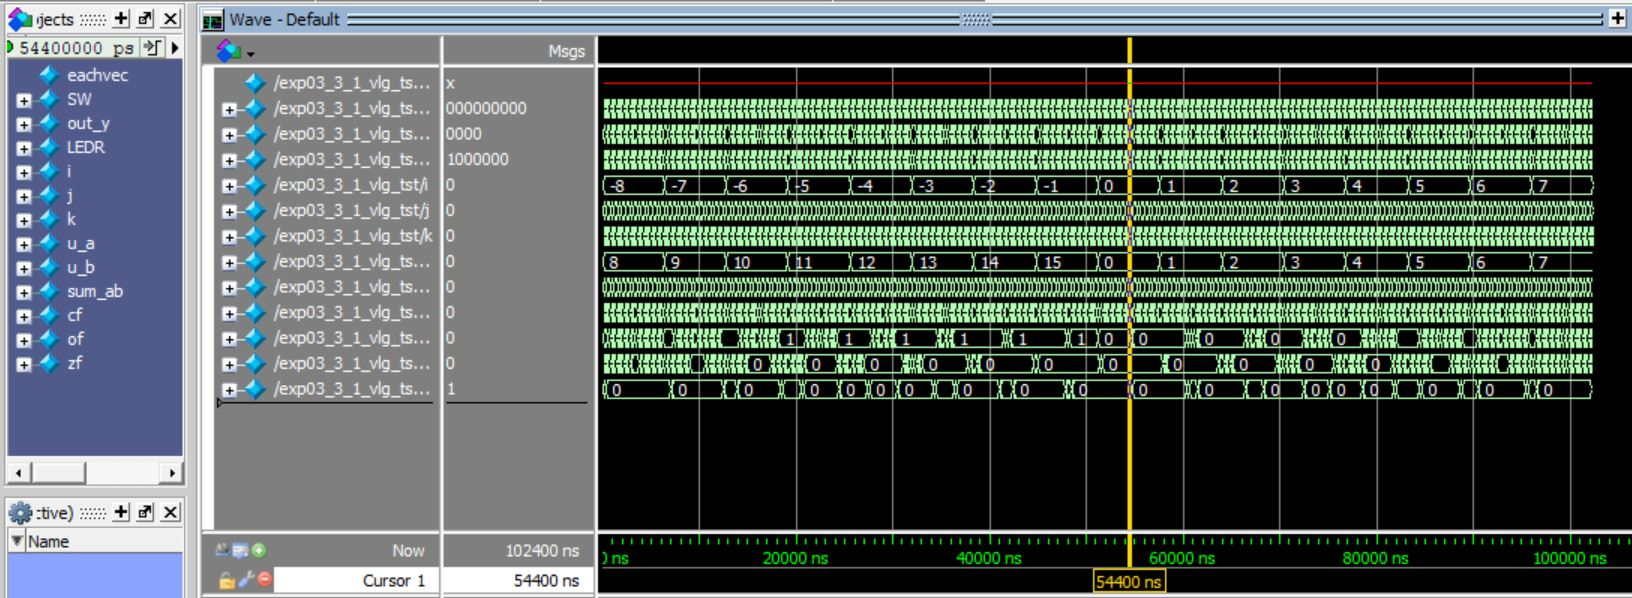
\includegraphics[width=0.8\textwidth]{03_3_1sim.JPG}
  \caption{运行仿真结果}
  \label{sim}
\end{figure}

\subsubsection{Verilog中的task}

因为实验题目中没有详细描述如何编写task,所以我现在
对task的基本运用做一些解释和补充。

task一般在测试文件进行编写,用于对主模块的测试。
task类似于函数,可以在initial程序块中调用它。传入到
task中的参数会按声明input的顺序接收。这些传入的参数与我们
要验证的正确值,也就是程序应该正确输出的值有关。我们在task中
将这些值与主模块输出的值进行比较,若不一样则通过display语句
把错误信息(在task中自行编写)输出出来。主模块输出的值不需要
在task中再次声明,因为这些值已经在测试模块开始处声明过了。

在initial程序块中一般会使用for循环,在循环体中产生
测试的输入(一些与循环变量有关的值),然后赋值给主模块的输入。
在赋值给输入以及计算要验证的正确值完成之后,应该调用task进行
测试,测试完成后进入下一个循环。

\subsubsection{思考题}
\begin{description}
  \item[思考题1] \hspace*{\fill} \\
        \hspace*{2em}判断溢出位时,应该比较操作数A1、B1和
        运算结果的符号位。因为进行加法时,A、B和A1、B1
        相同,但进行减法时,减数B会进行取反得到B1,
        再和A1(即A)相加再加1。而判断溢出是针对加法判断的,
        所以应该比较操作数A1、B1和运算结果的符号位
        (先在取反之后取符号位进行比较,这样之后再加1得到
        减数补码的原因,详见``实验原理''条目中对溢出位的解释)。
  \item[思考题2] \hspace*{\fill}
        \begin{itemize}
          \item 两种方法产生的运算结果一样,但
                进位位和溢出位不完全一样
          \item 方法一正确,方法二不完全正确
          \item 当进行加法时,两种方法结果一样,
                都是正确的
          \item 当进行减法且B=0时,方法二中第一行
                的运算$(\{n\{Cin\}\}$\^{}$ B) + Cin = 1111 + 0001$
                导致了进位,但这个进位信号并没有传递给
                进位位,因为上述加法赋给``t\_add\_Cin''
                的值是0000。这导致了进位位错误。
          \item 当进行减法且B=-8时,方法二中
                t\_add\_Cin的值是-8,符号位为1。
                而B求补之后所代表的应该是正数8,
                符号位应为0。这导致溢出位运算中
                t\_add\_Cin[n-1]的值(1)
                与实际值(0)不符,从而导致溢出位
                计算结果正好与实际值相反。\\
                分两种情况举例来说明。当A的符号位为0时,
                举例A=1。减法$1-(-8)=9=-7$转换成加法
                $1+8=9=-7$。两个正数相加得到负数,溢出。
                根据实验原理中溢出位的计算公式,若1与8的
                符号位相同且1与-7的符号位不同,则溢出。
                而这里1与8(即-8)的符号位不同,导致
                溢出位错误。\\
                当A的符号位为1时,举例A=-3。减法$-3-(-8)=5$
                转换成加法$-3+8=5$,一正一负相加不溢出。
                根据实验原理中溢出位的计算公式,若-3与8的
                符号位相同且-3与5的符号位不同,则溢出。
                而这里-3与8(即-8)的符号位相同,导致
                溢出位错误。
        \end{itemize}
  \item[思考题3] \hspace*{\fill}
        \begin{itemize}
          \item 一元约简运算:首先将运算符作用于操作数的
                第一位和第二位进行计算,再将运算符继续作用
                于得到的结果和第三位进行计算,
                以此类推直到最后一位
          \item 注意到这里不能用\&进行一元约简运算,
                因为有符号正数的符号位是0。如果用\&的话,
                所有的正数得到的结果都会是0
          \item 我认为一元约简运算更好,因为这样可以使用
                连续赋值语句并行计算,从而不用在过程语句中
                进行result与0的比较,这样可以提升效率
        \end{itemize}
\end{description}

\subsection{3.3.2 实现一个带有逻辑运算的简单ALU}
解决了有符号数补码的加减法运算,剩下的逻辑运算就相对简单了。
令A和B是输入的操作数,C是功能选择,输出为Y。先把每一种运算
的结果赋值给result0$\sim$result7,然后在always程序块中
利用case语句根据功能选择一个result输出。
\begin{lstlisting}[style=verilog-style]
module ALU_logical(A, B, C, Y);
	input [3:0] A, B;
	input [2:0] C;
	output reg [6:0] Y;
	wire [3:0] t_no_Cin;
	wire [6:0] result0, result1, result2, result3,
			result4, result5, result6, result7;
\end{lstlisting}
为了方便case语句的功能选择,我把实验3.3.1中的加减法运算代码
拆分开来,加法和减法分别连续赋值。
\begin{lstlisting}[style=verilog-style]
assign result0[4:0] = A + B;
assign result0[5] = (A[3] == B[3]) 
            && (A[3] != result0[3]); // overflow
assign result0[6] = ~(| result0[3:0]); // zero 

assign t_no_Cin = ~B;
assign result1[4:0] = A + t_no_Cin + 1; // {carry, result}
assign result1[5] = (A[3] == t_no_Cin[3]) 
            && (A[3] != result1[3]); // overflow
assign result1[6] = ~(| result1[3:0]); // zero
\end{lstlisting}
剩下的逻辑运算没有用到全部7个输出位,所以把不用的输出位赋值0
(代码省略)。然后分别用连续赋值语句赋值。
\begin{lstlisting}[style=verilog-style]
assign result2[3:0] = ~A;
assign result3[3:0] = A & B;
assign result4[3:0] = A | B;
assign result5[3:0] = A ^ B;
assign result6[0] = (A[3] == B[3] && A[2:0] > B[2:0]) 
	|| (A[3] == 0) && (B[3] == 1); // A > B
assign result7[0] = (A == B);
\end{lstlisting}
接下来就是写case语句把result赋值给Y(代码省略),编译
通过后用test bench写测试文件。测试代码相当于把
实验3.3.1的测试代码扩充一下,反正跑出来没啥问题,
就不贴代码了。
\begin{figure}[H]
  \centering
  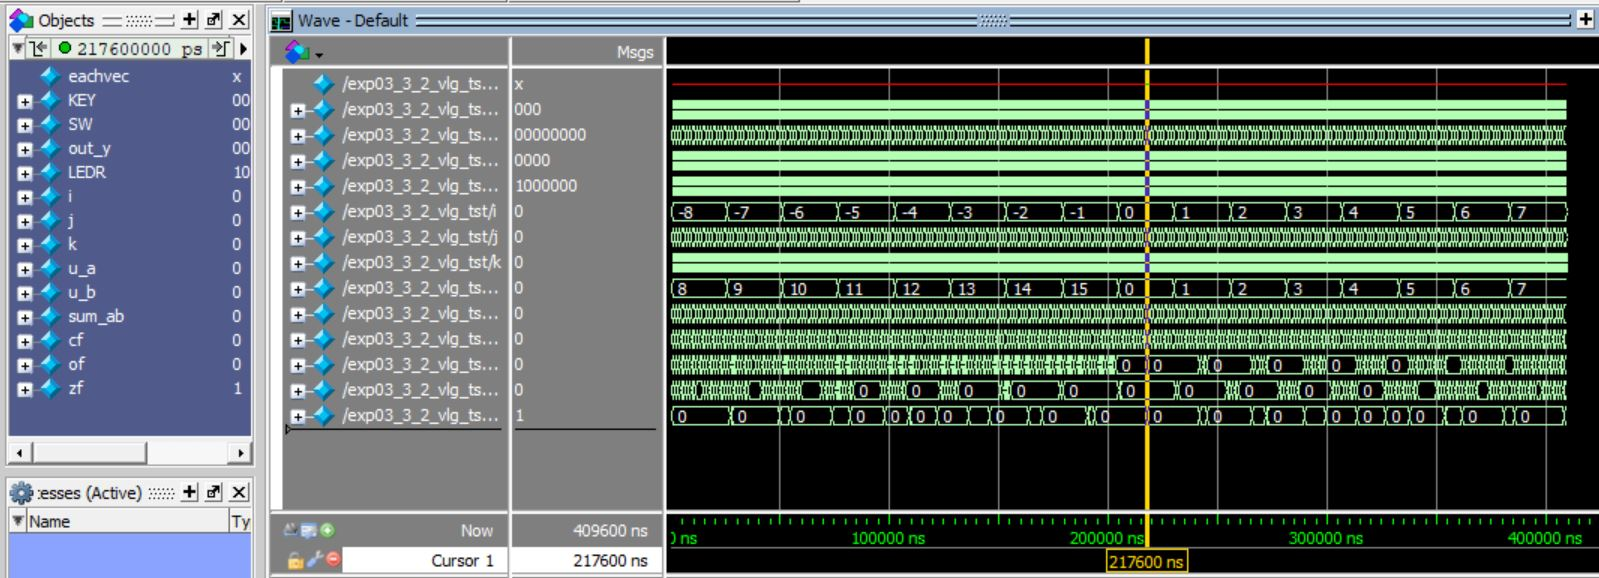
\includegraphics[width=0.8\textwidth]{03_3_2sim.JPG}
  \caption{运行仿真结果}
  \label{sim}
\end{figure}

\section{实验结果}
task测试成功,下载到开发板上运行也成功。两个实验圆满完成。
\begin{figure}[H]
  \centering
  \subfigure[实验3.3.1]{
    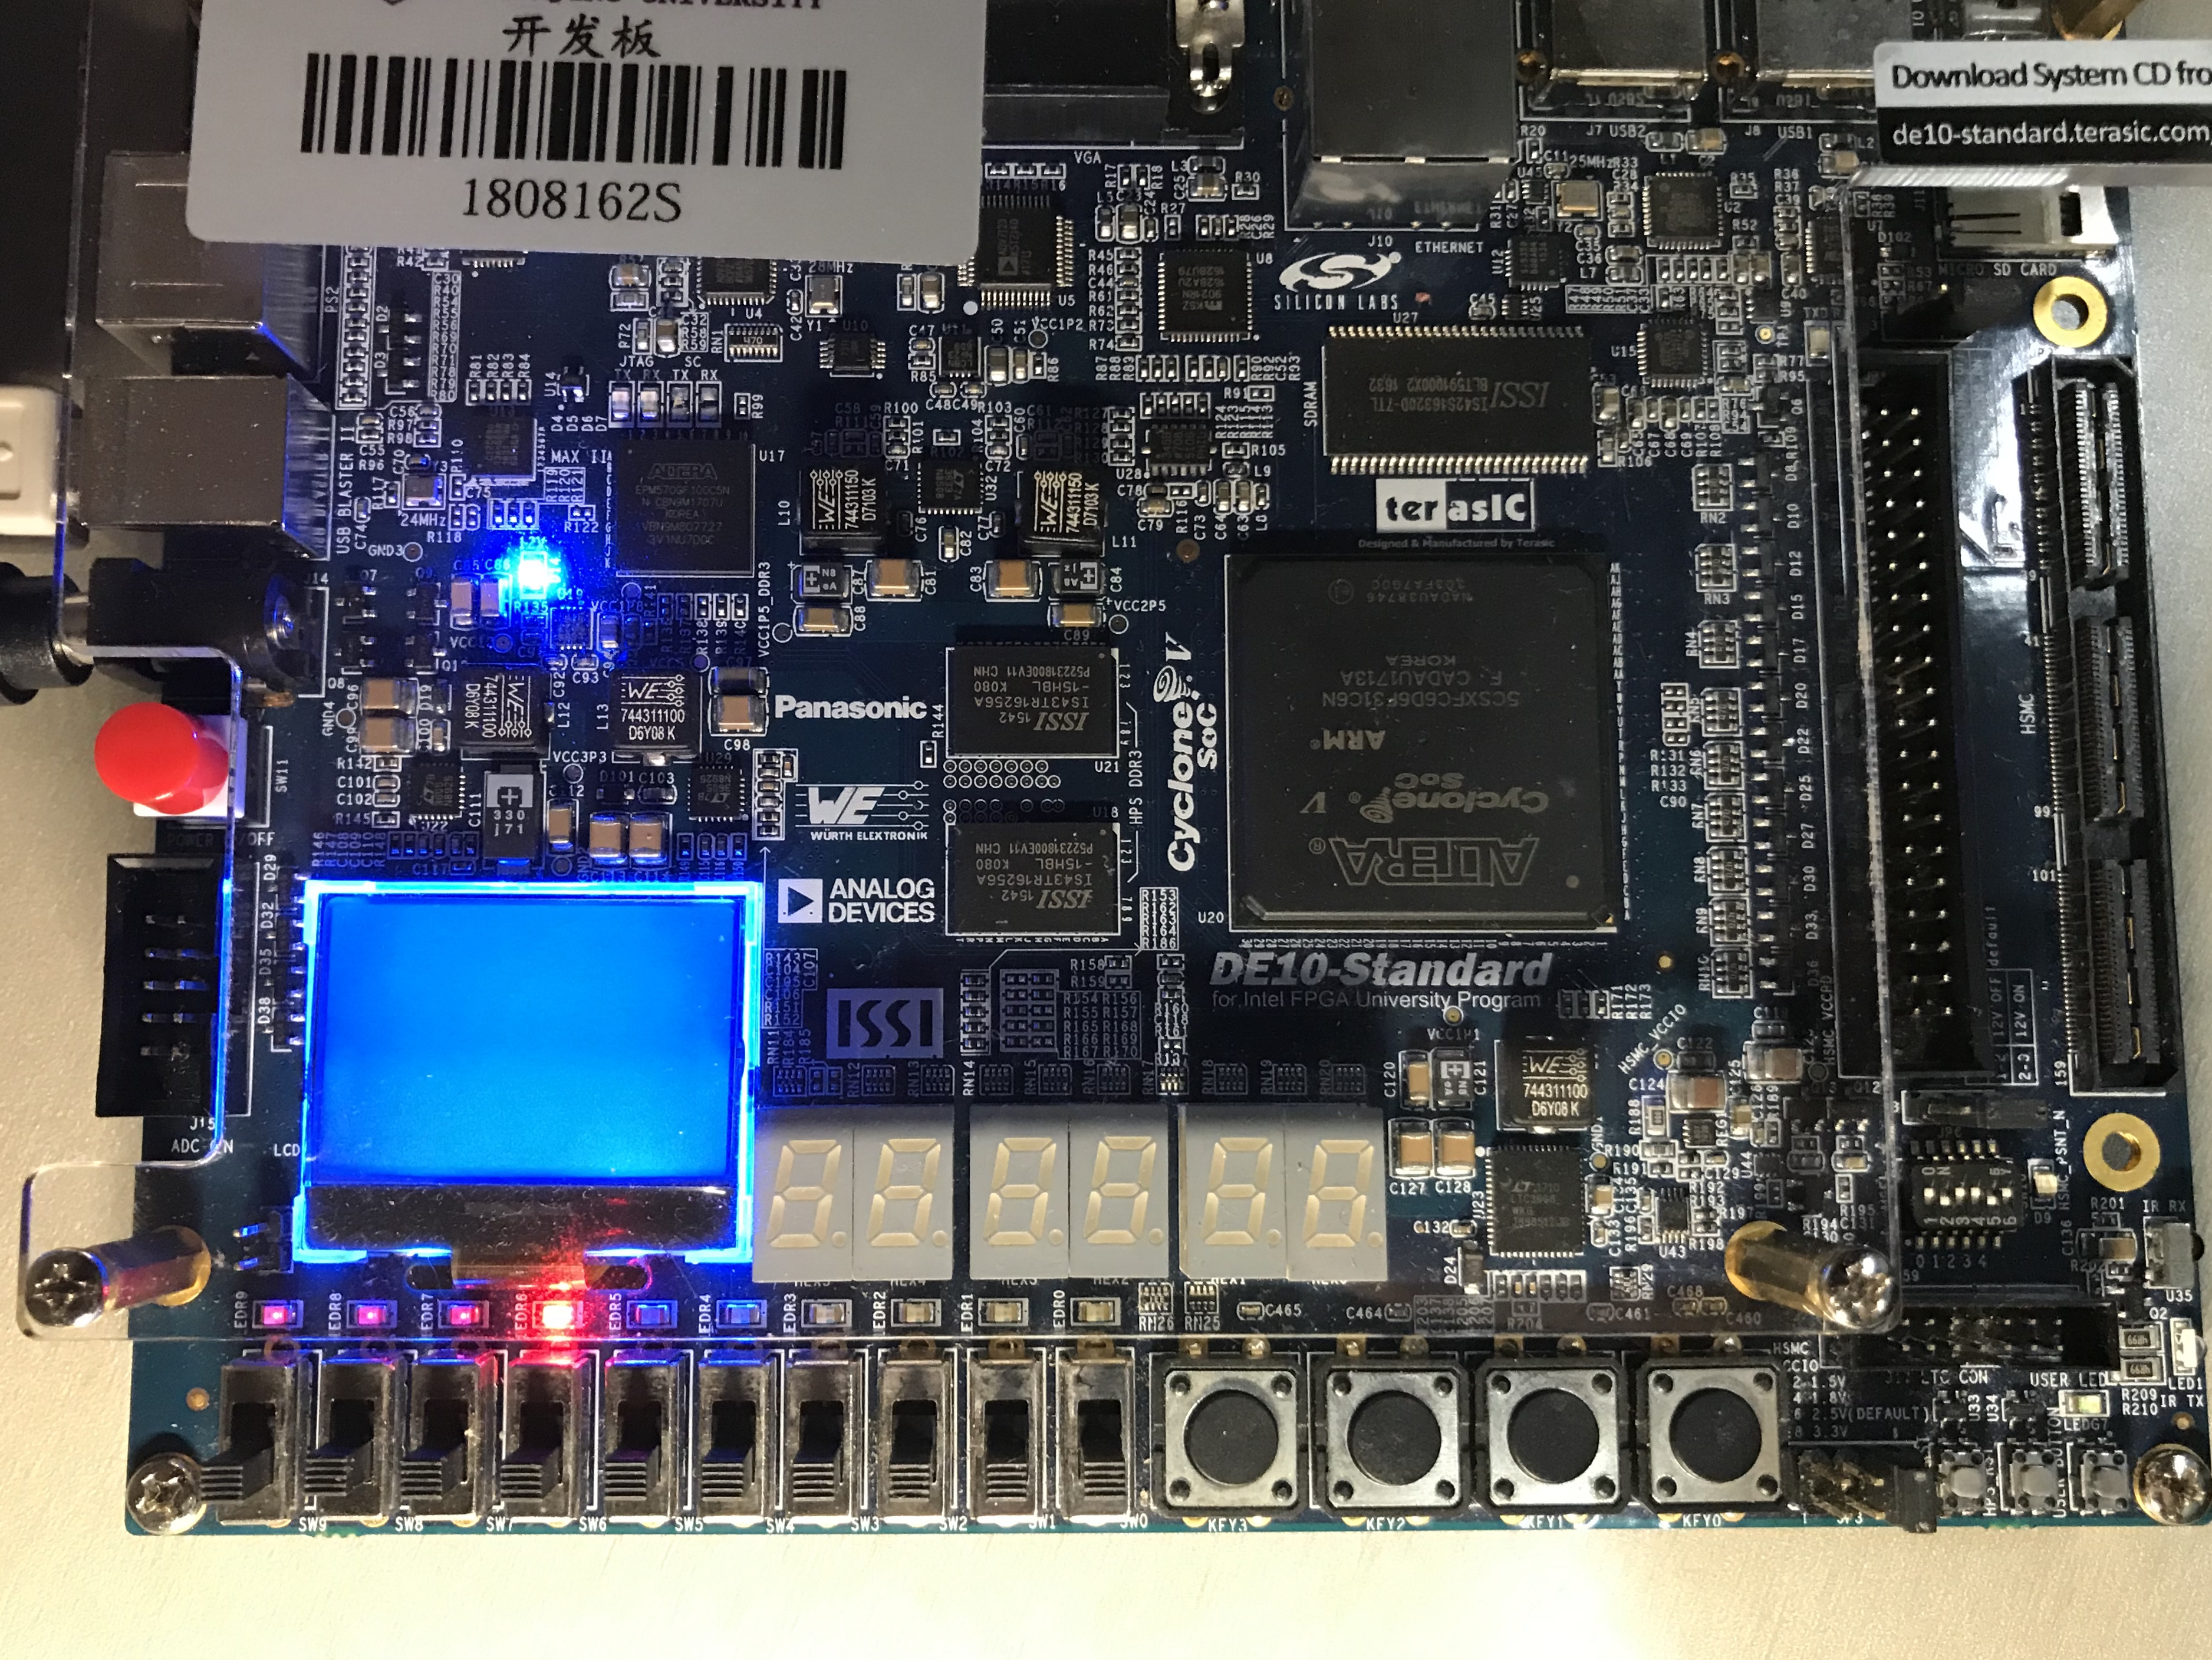
\includegraphics[width=0.45\textwidth]{fpga1.JPG}
  }
  \subfigure[实验3.3.2]{
    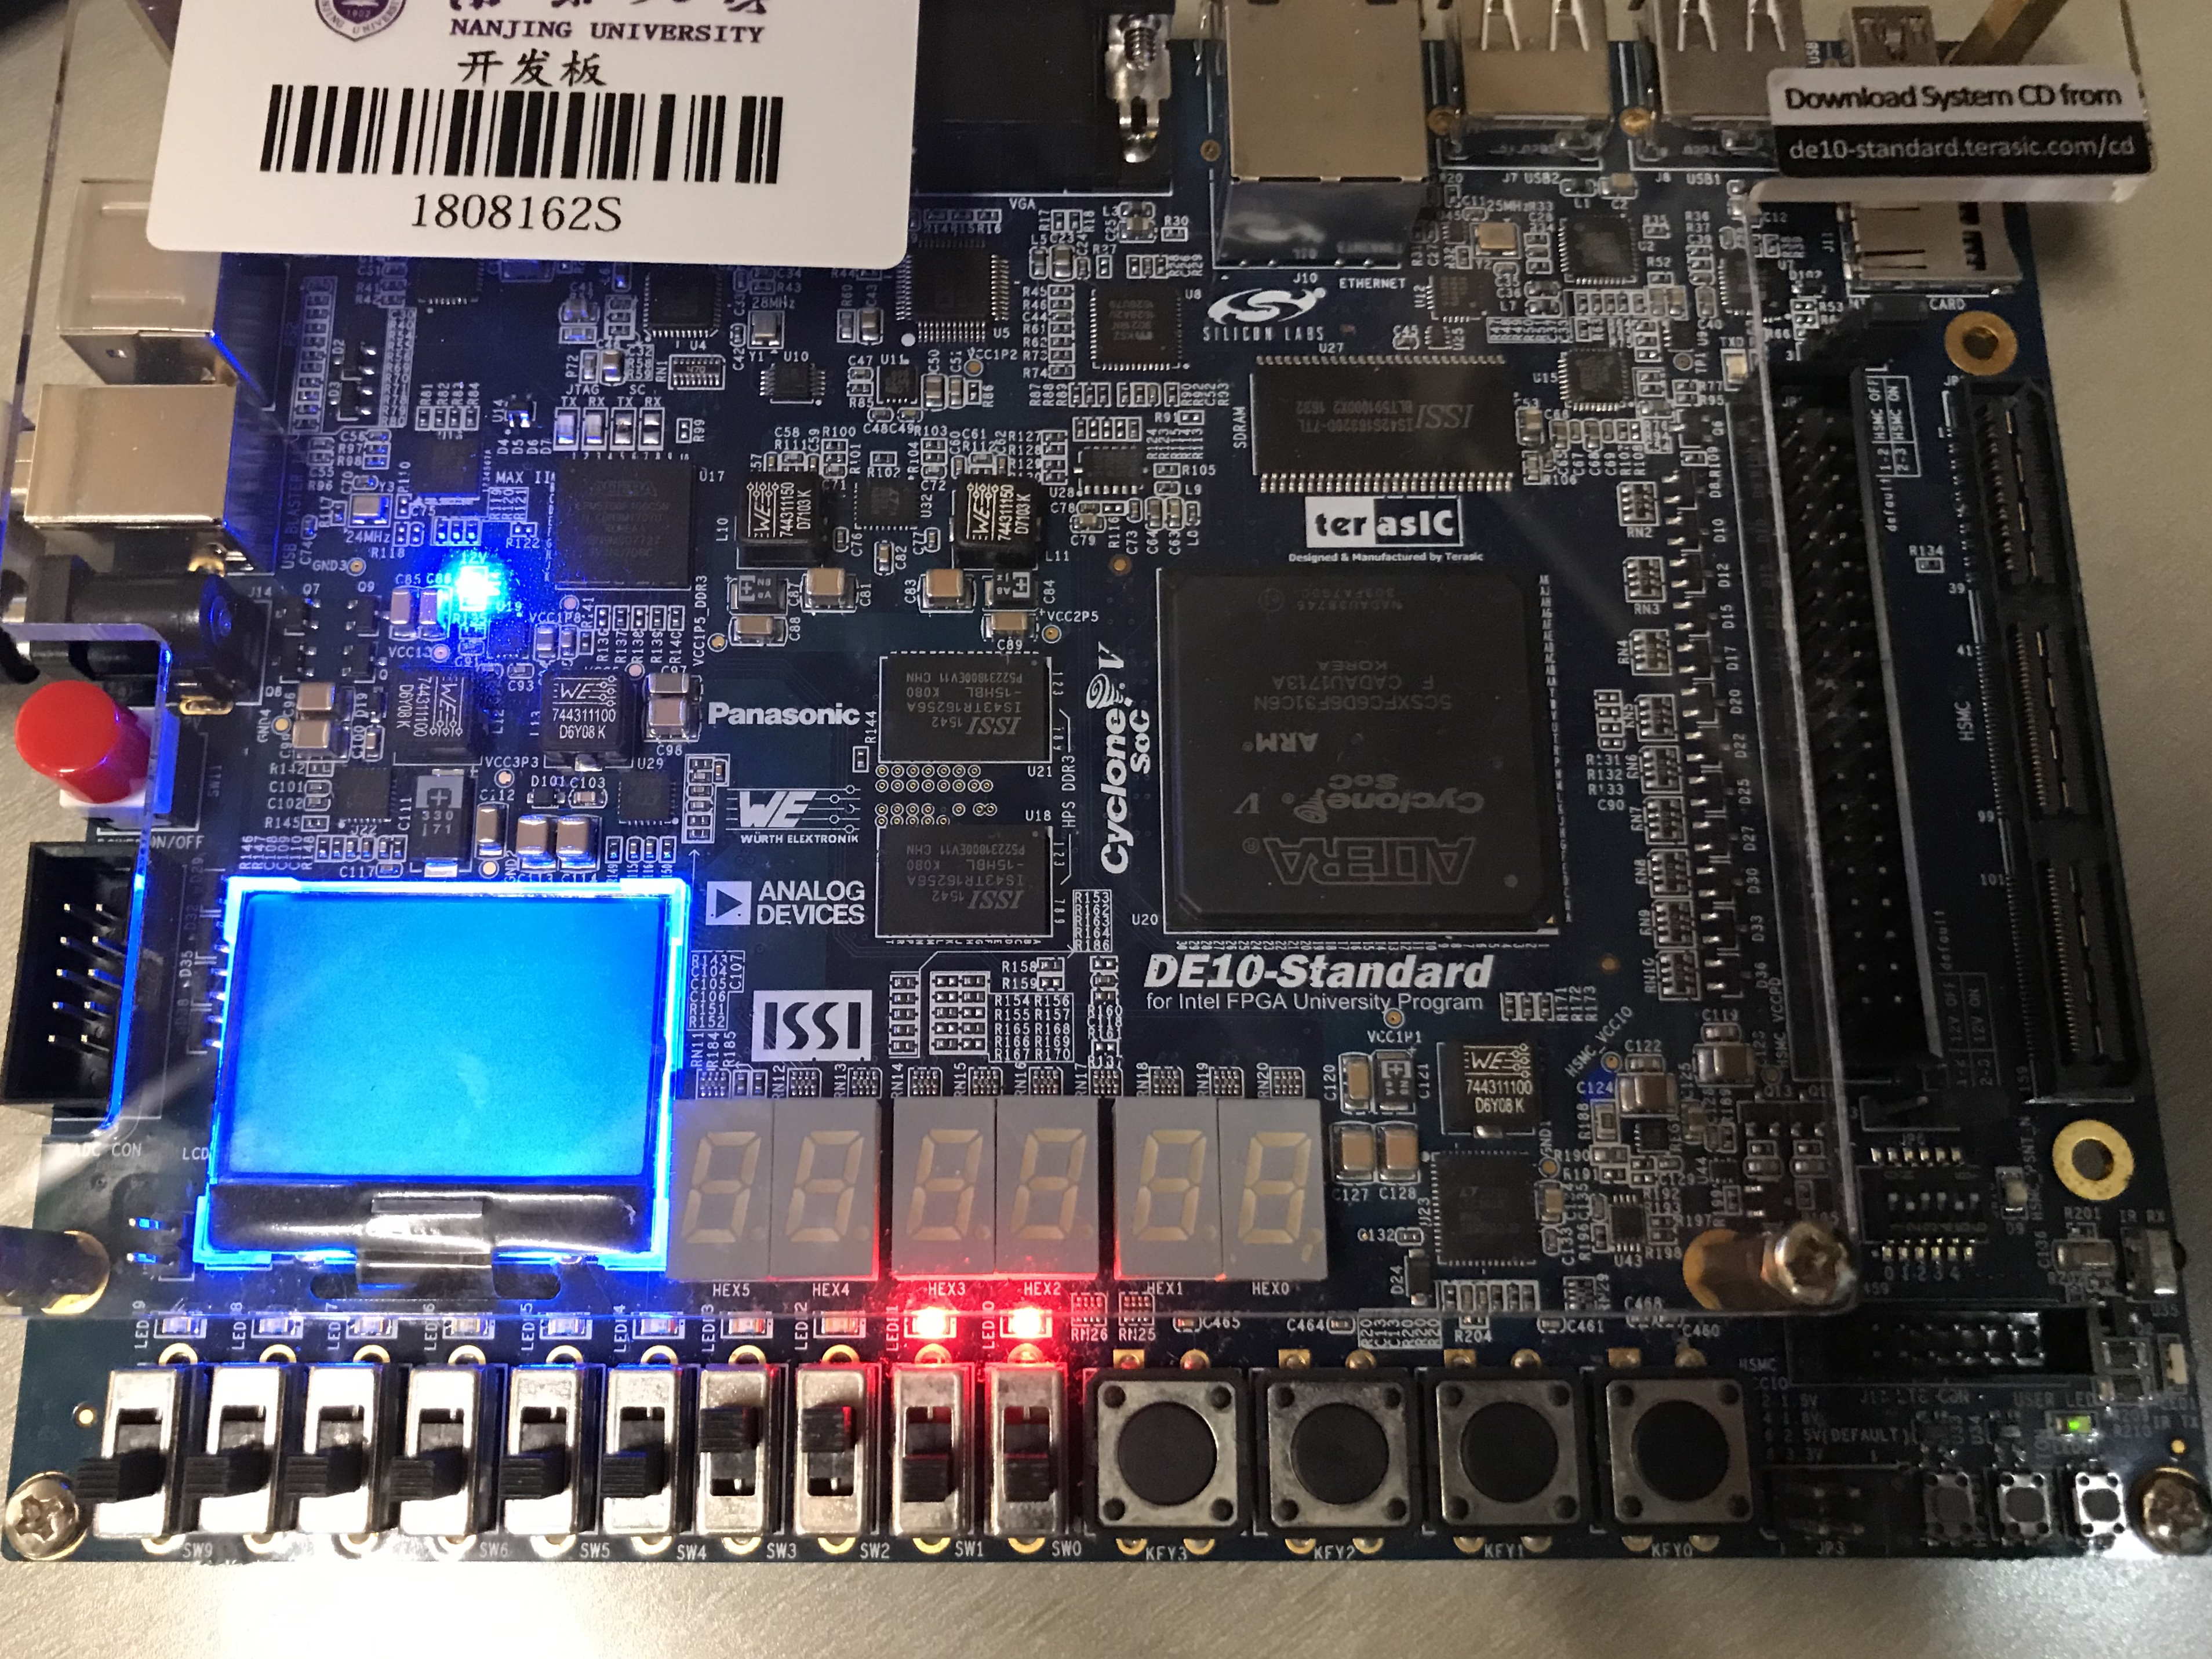
\includegraphics[width=0.45\textwidth]{fpga2.JPG}
  }
  \caption{下载运行}
  \label{fpga}
\end{figure}

\section{遇到的问题及解决办法}
\begin{itemize}
  \item 有符号补码的运算有亿点点烧脑,在查阅了课本以及
        《深入理解计算机系统》之后终于有了一点思路
  \item 问题:实验题目中没有给出编写task的详细教程。\\
        解决方法:仿照课本上的例子并结合实验题目
        摸索写法\sout{(连蒙带猜)}
  \item 在实验3.3.2写case语句的时候不小心把
        ``3'd数字''写成了``3'b数字'',想了好半天
        才发现这个bug……T\_T
\end{itemize}

\section{得到的启示}
\begin{itemize}
  \item n位数补码运算的测试样例先试$-2^{n-1}$和0
  \item 思维的漏洞还得靠测试样例来补救,思考题
        不能只靠思考,还需要在机器上实现并测试
  \item task应用在测试文件中效果不错,可以
        代替肉眼盯仿真波形图来进行测试
\end{itemize}

\section{意见和建议}
\begin{itemize}
  \item 可以在实验3.2叙述算术溢出之前先叙述一下
        Verilog中的有符号数和无符号数。我刚开始阅读
        该实验时并不能确定这是在讲述有符号数溢出还是
        无符号数溢出,读到后``两个正数相加结果为负''
        才能确定这是在叙述有符号数加法的溢出,
        希望可以在叙述溢出信号表达式的时候明确一下
        这是有符号数运算。
  \item 关于Verilog中有符号数和无符号数的话题,
        我从课本上的描述中稍微整理了一下:
        \begin{itemize}
          \item 默认把向量当作无符号整数处理
          \item 可以通过在声明中包含关键字``signed''
                声明一个有符号数,如``reg signed[15:0] A"
          \item 整型变量以及整型的纯文字总是被当作有符号数
          \item 如果在一个基数之前有一个字母``s''或``S'',
                那么其后的数字化文字会被当作有符号数,
                如``8'sb11111111'',其整数值为-1
          \item 仅当表达式中所有操作数都是有符号数时,
                才会采用有符号数补码的运算规则。否则,
                在计算表达式之前,所有有符号操作数都会
                被转换为无符号数
        \end{itemize}
  \item 实验3.3.1的task代码的第二行,应该是``input [3:0] results;''
\end{itemize}

\end{document}